\documentclass[twocolumn]{article}
\usepackage[utf8]{inputenc}
\usepackage[utf8]{inputenc}
\usepackage{graphicx} 
\usepackage[a4paper,top=2cm,bottom=3cm,left=2cm,right=2cm,marginparwidth=1.75cm]{geometry}
\usepackage{multicol}
\usepackage{amsmath}
\usepackage{xcolor}
\usepackage{hyperref}
\hypersetup{
    colorlinks,
    linkcolor={red!50!black},
    citecolor={blue!50!black},
    urlcolor={blue!80!black}
}
\usepackage{mathtools}
\usepackage{multirow}
\usepackage{dcolumn}
\usepackage{bm}

\title{\textbf{Summer Internship-2023}}
\author{Anantha Padmanabhan M Nair}
\date{\today}

\begin{document}

\maketitle



\section{Muons and their Properties}
Muons are unstable particles having intermediate mass between that of an electron and a proton, just like charged pions. Compared to pions, they are a little lighter.The muons carry one unit of electrical charge, either positive or negative, and are electrically charged. The life time of the muon is $2.2\mu s$

\subsection{Production of Muons}

\subsubsection{Atmospheric production of muons}
Muons that reach the surface of the Earth are indirectly produced when cosmic rays collide with atmospheric particles and produce decay products.Pions are produced when an atomic nucleus in the upper atmosphere is struck by a cosmic ray proton. These disintegrate within a few metres into muons, which are their preferred decay product, and muon neutrinos. 

\begin{equation}
    \pi^{\pm} \longrightarrow \mu^{\pm} + \nu_{\mu}
\end{equation}

The muons from these high-energy cosmic rays typically continue at a speed that is very close to the speed of light in the same general direction as the initial proton. 



\subsubsection{Production of Muons from Decay of Kaons}
Muons are also produced by the weak Deacy of the Kaons which is given by:
\begin{equation}
    K^{+} \longrightarrow \mu^{+} + \nu_{\mu}
\end{equation}

64\% of the time, disintegrates directly into $\mu^+$; 21\% of the time into $\pi^0$and$\pi^+$ and Only 6\% of the disintegrations produce three particles-$\mu^+$,$\mu^+$,$\mu-$. These pions then decay to produce muons according to:
\begin{equation}
    \pi^{+} \longrightarrow \mu^{+} + \nu_{\mu}
\end{equation}
\begin{equation}
    \pi^{-} \longrightarrow \mu^{-} + \Bar{\nu_{\mu}}
\end{equation}


\subsection{Decay of Muons}
The muons decay by the following scheme:
\begin{equation}
    \mu^{\pm} \longrightarrow e^{\pm} + \nu_{e} +\nu_{\mu}
\end{equation}


The nature of the muon decay has been studied by means of cloud chamber and by photographic emulsion methods.

\subsection{Properties of Muons}
The properties of the muons are shown in the table 


\begin{table}[ht]
    \centering
    \resizebox{0.85\columnwidth}{!}{%
    \begin{tabular}{|cc|c|}
        \hline
        \multicolumn{2}{|c|}{\textbf{Properties}}                           & \textbf{Values}              \\ \hline
        \multicolumn{1}{|c|}{\multirow{2}{*}{\textbf{Mass}}} & $m_{\mu}$    & $206.7686m_e$                \\ \cline{2-3} 
        \multicolumn{1}{|c|}{}                               & $m_{\mu}c^2$ & 105.659MeV                   \\ \hline
        \multicolumn{1}{|c|}{\textbf{Mean Life}}             & $\tau_{\mu}$ & $2.197 \mu s$                \\ \hline
        \multicolumn{1}{|c|}{\textbf{Spin}}                  & $s_{\mu}$     & 1/2                          \\ \hline
        \multicolumn{1}{|c|}{\textbf{Magnetic   Moment}}     & $\mu_{\mu}$  & $\frac{eh}{4\pi   m_{\mu} }$ \\ \hline
    \end{tabular}%
    }
    \caption{Properties of Muons}
    \label{muonproperty}
\end{table}






\subsection{How Does Muon reach the Earth Surface if its half life is 0.00156 ms}

We know that the half life of muons are $1.56\mu s$. But we are able to observe 
the muons coming from outer space on the earth surface. This is due to the relativistic
effects. Now we know that the total energy of the cosmic muon is in the range of 4GeV.
Let us calculate the value of $\gamma$. Considering the relativity:
\begin{equation}
    \gamma m_{\mu} c^2 =4GeV = 6.4\times10^{-10} J
\end{equation}

Substituting $m_{\mu} = 1.883 \times 10^{-28} Kg$ we get:
\begin{equation}
    \gamma = 37.754770
\end{equation}


NOw, let $t_{1/2}$ be the half life of muon when it is at rest WRT the earth and $t_{1/2}'$ 
be its half life when its moving. So, from time dilation, we have $t_{1/2}' =\gamma t_{1/2} $.
on substituting the values we get:
\begin{equation}
    t_{1/2}' \approx 0.058s
\end{equation}


As $\gamma$ is very high, the speed of the muons are very close to the speed of the
light. So time taken for the muons to reach the earth surface from the outer atmosphere is $\approx \text{distance}/c$
which is $\approx 10^{7}m/c \approx 0.03s$

So, this is why we are able to observe the cosmic muons incident on the earths surface
even if the half of the muons are in the range of micro seconds.




\section{Passage of Radiation Through Matter}

Naturally, penetrating radiation views matter as a collection 
of electrons and nuclei along with their subatomic particles, 
which are its fundamental building blocks. Reactions with the 
atoms or nuclei as a whole, or with each of their individual 
constituents, may take place through any channels that are permitted,
depending on the type of radiation, its energy, and the type of 
material. The Coulomb force, electromagnetic collisions with atomic 
electrons, elastic scattering from a nucleus, absorption in a 
nuclear reaction, and other processes can all occur when an alpha 
particle enters a gold foil, for instance. These occur with a 
certain probability that is determined by the fundamental 
interactions that are involved, as well as by the laws of quantum 
mechanics. 


\subsection{The Cross Section}

The crosssection is a common way to describe how two particles 
collide or interact. If the fundamental interaction between the 
particles is known, this quantity can be calculated and serves as a 
gauge of the likelihood that a reaction will take place. According 
to formal definitions, the cross-section is defined as follows. 
Think about a particle beam that hits a target particle 2, as 
seen in Fig. 2.1. Assume that the target is much farther away 
from the beam and that the beam's particles are evenly spaced out 
in time. After that, we can talk about a flux of Fincident particles 
per unit of space and time. 

Now, considering the amount of particles scattering into an angle 
$d\Omega$ per unit time, the number of particles is not constant if we 
measure more number of time. Let the average no of particles be $N_s$ and let F
be the flux. The differental crosssection is defined as :
\begin{equation}
    \frac{d\sigma}{d\Omega} (E,\Omega) = \frac{1}{F}  \frac{N_s}{d\Omega}
\end{equation}

that is, $d\sigma/d\Omega2$ is the average fraction of the particles scattered into df2 per unit time per
unit flux F. In terms of a single quantum mechanical particle, this may be reformulated
as the scattered probability current in the angle $d\Omega$ divided by the total incident
probability passing through a unit area in front of the target.


\begin{figure}[ht]
    \centering	
     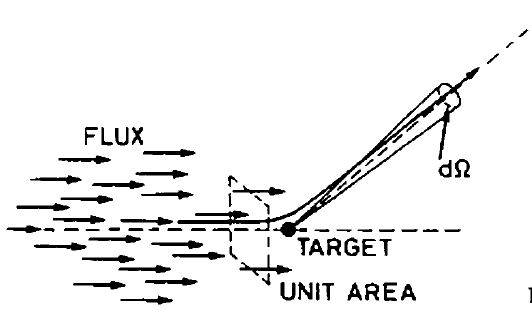
\includegraphics[width=\columnwidth]{crossection.png}
     \caption{CDiagram showing the  crosssection}
     \label{CSdiag}
\end{figure}

So, the total crosssection is given by:

\begin{equation}
    \sigma(E)=\int d \Omega \frac{d \sigma}{d \Omega}
\end{equation}


Assuming that the target centers are uniformly distributed and 
the slab is not too thick so that the likelihood of one center sitting 
in front of another is low, the number of centers per unit perpendicular 
area which will be seen by the beam is then $N\delta x$ where N is the 
density of centers and $\delta x$ is the thickness of the material along 
the direction of the beam. If the beam is broader than the target and A is 
the total perpendicular area of the target, the number of incident particles 
which are eligible for an interaction is then FA. The average number scattered 
into $d\Omega$ per unit time is then:

\begin{equation}
    N_s(\Omega) = FAN\delta x \frac{d\sigma}{d\Omega}
\end{equation}

and,

\begin{equation}
    N_{tot} = FAN \delta x \sigma
\end{equation}

And the probability of interaction in $\delta x$ is $N\sigma \delta x$

\subsection{Interaction Probability}

Here we will caclulate what id probability that a particle does not involve
in an interaction for a distance of x, this probability is known as the 
survival probability $P(x)$. Let the probability of having an interaction between 
$x$ and $dx$ be $wdx$. Then we have the probability of not having an interaction
between $x$ and $x+dx$ as:

\begin{equation}
    P(x+dx) = P(x)(1-wdx)
\end{equation}

On solving, we get the P(x) as :
\begin{equation}
    P(x) = C\exp{-wx}
\end{equation}
C turns out to be 1 while substuting the usual probability properties.


Now as we have the interaction probability, we will calculate the mean free
path, which is defined as:
\begin{equation}
    \lambda = \frac{\int x P(x)dx}{\int P(x)dx} = \frac{1}{w}
\end{equation}

but the interaction probability depends on the $\delta x$ intuitively, after 
approximating to the linear order terms we get:
\begin{equation}
    \lambda = \frac{1}{N\sigma}
\end{equation}


So the survival probability becomes:

\begin{equation}
    P(x) = \exp{(\frac{-x}{\sigma})}=\exp{(-N\sigma x)}
\end{equation}



\subsection{Energy Loss of the penetrating particle by Atomic Collisions}

Inelastic collisions with atomic electrons and the elastic scattering from the nuclei
are the two main reasons for the energy loss and change in direction of the particle.

Of course, the inelastic collisions are statistical in nature and have a 
certain quantum mechanical probability of happening. The fluctuations in 
the total energy loss are, however, small due to their abundance per 
macroscopic pathlength, so one can effectively work with the average 
energy loss per unit path length. Bohr first calculated this quantity 
often referred to as the stopping power or simply dE/dx—using classical 
reasoning. Later, Bethe, Bloch, and others did so using quantum mechanics.


\subsubsection{Bohr's Calculation}

Consider a heavy particle travelling through a material medium with a 
charge ze, mass M, and velocity v. Assume that an atomic electron is 
present at a distance and from the particle trajectory as shown in 
Figure-\ref{bohrsct1} 
In order to capture the electric field acting 
on the electron at its initial position, we assume that the electron 
is free, initially at rest, and that it only moves very slightly during 
the interaction with the heavy particle. Furthermore, because of its much 
greater mass (M>m), we assume that the incident particle will have 
essentially maintained its original course after the collision. 
This is one justification for separating heavy particles from electrons!




\begin{figure}[ht]
    \centering	
     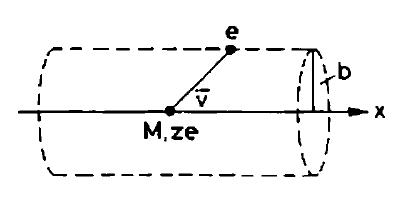
\includegraphics[width=\columnwidth]{bohrsct.png}
     \caption{Diagram For Bohr Calculation of Scattering}
     \label{bohrsct1}
\end{figure}


Now, we will calculate the energy gained by the electron by finding the momentum impulse
it receieves by colling with the heavy particle.so:
\begin{equation}
    I = \int F dt = e\int E_{\perp} dt =e\int E_{\perp} \frac{dx}{v}
\end{equation}



By applying the gauss law, we get,

\begin{equation}
    \int E_{\perp} 2\pi bdx = 4\pi ze 
\end{equation}

So that we have:

\begin{equation}
    I = \frac{2ze^2}{bv}
\end{equation}

The energy gained by the electron is then:
\begin{equation}
    \label{eq1}
    \Delta E(b) = \frac{I^2}{2m_e} \frac{2z^2e^4}{mev^2b^2}
\end{equation}

Now, let the density of particles be $N_e$, then the energy lost to all the electrons
in the range b to b+db is given by:
\begin{equation}
    -dE(b) = \Delta E(B) N_e dV = \frac{4\pi z^2e^4}{mev^2} N_e \frac{db}{b} dx
\end{equation}

On solving with volume element $dV = 2\pi b db dx$ we get:

\begin{equation}
    -\frac{db}{dx} = \frac{4\pi z^2 e^4}{m_e v^2}N_e \ln{(\frac{b_{max}}{b_{min}})}
\end{equation}

Ideally the limit should be 0 to infinity, but due to our assumption that
the collision at large b wont take place over a short period of time, there is an upper bound
$b_{max}$ and also at b=0, the integral diverges so there is also a $b_{min}$.

To calculate the $b_{min}$, the maximum kinetic energy is transfered when there is
a headon collission and the maximum energy it can gain is $\frac{1}{2}m_e (2v)^2$,
taking relativity we get this energy as $2\gamma^2 m_e v^2 $
substuting this to Equation-\ref{eq1}, we get,
\begin{equation}
    b_{min} = \frac{ze^2}{\gamma m_e v^2}
\end{equation}









\section{Simuation Using Geant4}

The detection of the cosmi muons using the ALICE detectors is being
simulated using the Geant4 tooklit. The details about the geometry construction
and the particles will be discussed below.


\subsection{Detector Geometry}

The detectors used here are one honeycomb ALICE detector placed 
between 2 scintillation detectors. The honeycomb detector is madeup of 1024 HExagonal units in a 
$32\times32$ manner. The Radius and the height of the Hexagon is 5mm and length of the scintillation detector
is same as that of the length of the honeycomb detector. The Distance between the Two scintillation
detectors is 1m. And the dimentions of the world volume is $2.5m\times2.5m\times2.5m$

\end{document}
